\section{Introduction}
  In~\autoref{chap:preliminaries}, we have defined the main notions we will use
  thoughout this thesis and we have presented common ways to numerically
  represent linguistic information. A common method used in the literature is
  \textit{word embeddings}: it consists of associating a real-valued vector to
  each word of a vocabulary. This vectorial representation of words benefits
  from the mathematical properties of vector spaces. It allows one to perform
  operations on vectors and compute distances between them, which are the main
  requirements for downstream models to be able to use word embeddings to solve
  NLP tasks. We have seen that word embeddings need to have vector values which
  reflect the linguistic properties of words so downstream models can have
  access to linguistic knowledge through the use of word embeddings, but we have
  not yet explained how the values of word embeddings are chosen neither how
  word embeddings are actually used to solve downstream NLP tasks. \medskip

  In the early works on word representations, values of vectors were chosen
  based on linguistic and lexical properties of
  words~\citep{osgood1964semantic,bierwisch1970classifying} . For example, the
  first value of each word embedding could be an integer representing the nature
  of the word ($1$ for nouns, $2$ for verbs, $3$ for adjectives, etc.), the
  second value could be the ratio between the number of times a word is used as
  the subject and as a complement in a text, etc. While those choices are
  appropriate from a linguistic point of view because it makes sense to directly
  incorporate properties of words into their vector representations, it is not
  appropriate from a scaling point of view. Indeed, the number of words in a
  language is large (it can reach several millions when we consider that
  entities like cities, regions, brands, etc. can occur in a text and therefore
  can be an element of the vocabulary of a language), so the process of
  identifying and generating handcrafted linguistic properties of words to
  incorporate them into their word vector becomes a long and complex task.
  Moreover, this process requires the knowledge of linguistic experts, which is
  expensive and time consuming because it requires human manual annotations.
  \medskip

  To overcome the problem of manual labor required by handcrafted features, NLP
  scientists sought to use methods from the field of \textit{Machine Learning}
  (ML) to produce them automatically. Machine learning is a subfield of
  artificial intelligence that aims to create algorithms or statistical models
  which can identify and extract information from data without being explicitly
  programmed to. Machines use data to \textit{learn} rules about the
  information hidden inside it. Machine learning algorithms and models are then
  used in different kinds of task like identifying the model of a car from a
  picture of it, detecting abnormal behavior of people in videos or predicting
  the power consumption of a city for the next week. Advances in computing power
  available in machines have allowed to build more complex models over the
  years~\citep{taigman2014deepface, silver2016mastering, devlin2019bert}.\\

  In this chapter,~\autoref{ch02:sec:supervised-unsupervised} presents the
  different types of machine learning algorithm that exist while
  \autoref{ch02:sec:training-model} explains how can a machine \textit{learn}
  from data. Lastly,~\autoref{ch02:sec:ml-for-we} details some of the main
  machine learning models used for dealing with word embeddings. This section
  (\autoref{ch02:sec:ml-for-we}) will also serve as a foundation for the rest of
  this thesis as the contributions described in this thesis use those machine
  learning models.

\section{Supervised and unsupervised learning}
  \label{ch02:sec:supervised-unsupervised}
  As said in the previous section, machine learning algorithms use data to
  extract, by themselves, rules about the information contained inside data in
  order to solve a given problem. These algorithms are able to perform on their
  own the information extraction operation to solve the problem, without needing
  to follow a computer program that indicates precisely where is the information
  contained inside data which is relevant to the given task. However, some
  machine learning models need some help at the beginning of the extraction
  process to \textit{learn}, \textit{i.e.} to understand what information is
  required to solve the task and what rules need to be designed to extract
  it. \medskip

  Let us take a small example to illustrate this. Let say we want to know if a
  mushroom is edible or poisonous based on a picture of it and that we want to
  use a machine learning algorithm to solve this problem. If enough pictures of
  mushrooms are given to the algorithm, it will be able to recognize some common
  patterns in certain types of mushrooms (the color of the cap, the spacing in
  the gill etc.) and it will be able to group together mushrooms with similar
  features. However, if no one has indicated for each picture (\textit{i.e.} the
  data) if it is a poisonous or an edible mushroom, then the algorithm cannot
  guess the correct answer and therefore cannot differentiate edible from
  poisonous mushrooms. Thus, without any help, the machine learning algorithm
  cannot learn to correctly predict if a mushroom is edible or not. The same
  thing also happens in the NLP domain. For instance, if an algorithm has to
  predict the subject of a news article (like ``sport'', ``economy'' or
  ``politics'') and no one has helped the algorithm by associating articles with
  their subject, then the algorithm has no way to learn what are the common
  features of sport articles because it cannot know which articles are sport
  articles. The process of adding a hint to help the algorithm to differentiate
  edible from poisonous mushrooms is called \textit{annotating} data. Each piece
  of data (\textit{i.e.} each picture of a mushroom) is associated to a
  \textit{label} (\textit{i.e.} the hint) which indicates if the mushroom is
  edible or not. With this example, we can separate machine learning algorithms
  into two groups:

  \begin{enumerate}
    \item When the algorithm needs a hint or additional knowledge to be able to
      learn how to differentiate different categories of objects in data (like
      predicting the toxicity of a mushroom) we call it \textit{supervised
      learning}.
    \item When there are no hints available and the objective of the algorithm is
      to group together or to find common patterns and features in data, we call
      it \textit{unsupervised learning}.
  \end{enumerate}

  \noindent This section presents supervised learning
  in~\autoref{ch02:subsec:supervised-learning} and unsupervised learning
  in~\autoref{ch02:subsec:unsupervised-learning}. Another type of machine
  learning algorithm called \textit{semi-supervised learning} which lies between
  supervised and unsupervised learning is presented
  in~\autoref{ch02:subsec:semi-supervised-learning}.

  \subsection{Supervised learning}
    \label{ch02:subsec:supervised-learning}
    In supervised learning, each piece of data is annotated with one or several
    labels (in the mushroom example, the annotation to indicate if the mushroom
    is edible or poisonous is a single label). Machine learning algorithms learn
    how to use the features of data (\textit{i.e.} the information contained
    inside it) to predict the corresponding label(s). Data can have many forms:
    an image, a video, a list of numerical values to indicate the properties of
    a person or an object, etc. Labels can also be of different types: an
    integer (\textit{e.g.} when predicting an age), a word (\textit{e.g.} when
    predicting the species of an animal), a real value (\textit{e.g.} when
    predicting a temperature), etc. In machine learning, we use the notion of
    \textit{input} to designate data given to algorithms and \textit{output} to
    designate the prediction of algorithms~\citep{ayodele2010types}. In the case
    of supervised learning, the model learns how to map the input to the
    corresponding correct output. After the \textit{learning phase} (also
    called the \textit{training phase}) which consists in finding the mapping
    function that correctly predicts the output given the input, the algorithm
    is fed with new input data it has never seen (and for which we do not know
    the corresponding label) and uses what the model has learned to predict the
    output. This prediction step on new data is the \textit{inference
    phase}. In the small mushroom example, this step consists in using the
    trained model to know if a mushroom is edible or not from a new picture of
    mushroom (\textit{i.e.} a picture not used during the learning phase).
    We can formalize supervised learning with mathematical terms:

    \theoremstyle{definition}
    \begin{definition}[Supervised learning]
      Let $\mathcal{X} \subseteq \mathbb{R}^d$ be the vector space containing
      input data, $\mathcal{Y}$ the label space containing output labels and
      $\mathcal{S}$ a set of annotated examples of the form $(\mathbf{x}_i, y_i)
      \in \mathcal{X} \times \mathcal{Y}$ where $\mathbf{x}_i$ is the feature
      vector of the $i$-th example and $y_i$ its corresponding output label. A
      supervised learning algorithm searches a function $f: \mathcal{X} \to
      \mathcal{Y}$ among the space of hypothesis $\mathcal{H} =
      \mathcal{Y}^\mathcal{X}$ which gives the same (or the closest) output
      value $f(\mathbf{x}_i)$ as $y_i$ for all $(\mathbf{x}_i, y_i) \in
      \mathcal{S}$.
    \end{definition}

    The label space $\mathcal{Y}$ depends on the task solved by the
    machine learning algorithm.~\autoref{ch02:tab:label-space} reports some
    examples of common label spaces used in supervised learning tasks.

    \begin{table}[h]
      \centering
      \resizebox{\textwidth}{!}{
        \begin{tabular}{lll}
        \toprule[0.15em]
        Type of task & Label space & Example of a task \\
        \midrule[0.08em]

        Binary classification &
        $\mathcal{Y} = \{0, 1\} \text{ or } \mathcal{Y} = \{-1, +1\}$ &
        Predict if a mushroom is edible (+1)\\
        &&or not (-1).\\
        &&\\ % empty row

        Multi-class classification &
        $ \mathcal{Y} = \{1, 2,~\ldots~, K\}$ &
        Predict the species of an animal\\
        &&among $K$ possibilities ($1$ = ``dog''; \\
        &&$2$ = ``cat''; \dots).\\
        &&\\ % empty row

        Regression &
        $ \mathcal{Y} = \mathbb{R} $ &
        Predict a temperature.\\
        \bottomrule[0.15em]
      \end{tabular}}
      \caption{Examples of label spaces for different supervised learning
      tasks.}
      \label{ch02:tab:label-space}
    \end{table}

    Many NLP tasks can be solved with supervised learning. Here is a
    non-exhaustive list of examples:

    \begin{itemize}
      \item Text classification and sentiment analysis (described
        in~\autoref{ch01:subsec:extrinsic-evaluation}
        of~\autoref{chap:preliminaries}) can be both solved with supervised
        learning. Input data are commonly vector representations of texts or
        sentences and output labels can either be a word to indicate the
        category of the text, or an integer to indicate the number of rating
        stars associated to a comment.
      \item Automatic translation is another example of task that can be solved
        with supervised learning. The machine learning algorithm is fed with a
        sentence from a specific language, and the output is the sentence
        translated into another language. The algorithm learns how to map the
        two sentences together and therefore, learns how to translate sentences.
      \item In a textual entailment task (which consists in predicting if two
        sentences are related by a cause/consequence relation or if they are
        unrelated), input data are the two sentences (or the vector
        representations of sentences) and output labels are binary values that
        indicate if the two sentences are related or not.
    \end{itemize}

  \subsection{Unsupervised learning}
    \label{ch02:subsec:unsupervised-learning}
    The main difference between supervised and unsupervised learning is that
    there are no labels in the case of unsupervised learning (or from a
    different point of view, because data do not have any annotations nor labels, we
    cannot use supervised learning algorithms so we have to rely on
    unsupervised learning methods). Two main tasks can be solved with
    unsupervised learning: clustering and data transformation. Let us describe
    and illustrate those tasks with NLP examples.

    \begin{itemize}
      \item \textbf{Clustering}. Clustering is the task of grouping similar
        objects into sets (called \textit{clusters}) such that two objects from
        the same cluster are more similar to each other than to objects from
        another cluster. Clustering cannot be solved with supervised learning
        algorithms because there are no labels to indicate in which cluster each
        object should belong. Information contained inside data needs to be used
        to find which objects are similar together.

        Clustering can be used in NLP to analyze comments posted on social media
        platforms. While each user is unique, we can group together people with
        similar behavior because they either speak about the same subjects or
        have the same style of writing. This kind of data do not have any
        labels: there are no extra information in a comment to indicate in which
        group a user belongs nor to indicate how many groups may exist.
        Clustering can be used to group together comments and detect some common
        patterns between users.

      \item \textbf{Dimensionality reduction}. Dimensionality reduction is the
        task of transforming data to reduce the number of features or the number
        of dimensions in vectors. For some data, the number of features or
        dimensions can be very large (in the order of thousands) which makes
        them unsuitable for use in supervised learning algorithms. There are no
        labels or annotations to indicate which dimensions would be the most
        useful for a given task so unsupervised learning algorithms are used to
        find them automatically.~\autoref{chap:methods-reduction} focuses on
        presenting the most common methods that exist to reduce the number of
        dimensions in word embeddings.

        In document classification, data can be expressed by vectors of
        thousands of dimensions with many values set to 0 and a few values set
        to 1 (we call them \textit{sparse vectors}). Such vectors can be
        obtained by checking the presence/absence of many words in a news
        article or in a website. Large sparse vectors can be difficult to use in
        supervised learning models because of the numerous 0 so vectors are
        usually transformed into \textit{dense vectors}, \textit{i.e.} vectors
        of continuous real values with a smaller number of dimensions. There are
        no labels in this kind of data to indicate what are the transformation
        to apply, so unsupervised learning algorithms have to learn them by
        themselves.
    \end{itemize}

  \subsection{Semi-supervised learning}
    \label{ch02:subsec:semi-supervised-learning}
    Semi-supervised learning is another type of machine learning which is
    between supervised and unsupervised learning. In semi-supervised learning,
    only a small amount of data have labels; the majority of data is unlabeled.
    Semi-supervised learning algorithms use a combination of supervised and
    unsupervised algorithms to solve a given task. For example, one can use
    clustering to group together similar objects and then propagate the
    annotations of labeled objects of a cluster to unlabeled objects of the same
    cluster. \medskip

    Semi-supervised learning is often used in NLP. As we have seen
    in~\autoref{chap:preliminaries}, annotating each text or each word of a
    large vocabulary with its linguistic properties is a difficult and
    time-consuming task because it requires the knowledge of linguistic experts.
    The small amount of labeled data is used to either assume the properties of
    similar items or to propagate the annotations to unlabeled data. For the
    task of learning word embeddings which encode linguistic information, vector
    representations of words are learned with unsupervised learning algorithms
    which use a small amount of supervision with either a few number of
    annotated examples of similar words or with an hypothesis about the
    distribution of semantic knowledge in a language. \autoref{chap:methods-we}
    presents the most common methods to learn word embeddings; most of them are
    semi-supervised algorithms.

\section{Training a machine learning model}
  \label{ch02:sec:training-model}
  Machine learning models learn to identify patterns and infomation inside data
  and in the case of supervised learning, learn how to predict an output label
  given input data.  Models learn without being explicitly programmed to:
  information is usually hidden inside the numerical representation of data,
  which prevents developers to create specific rules that extract only some of
  the values in data and then combine them with a manually-written formula to
  make predictions.  Yet, machine learning models are able to automatically
  extract useful information from data needed to solve a given task and learn
  how to combine these informative values to predict the correct output label.
  This automatic process of learning is the result of setting an objective for
  the algorithm (\autoref{ch02:subsec:objective-function}) and giving it tools
  to achieve it (\autoref{ch02:subsec:gradient}).

  \subsection{Objective function}
    \label{ch02:subsec:objective-function}
    In supervised learning, since each data is associated with an output label,
    the goal of the algorithm is pretty intuitive: being able to predict the
    correct label for each example. We can modelize this goal in mathematical
    terms with the notion of a \textit{loss function}.

    \theoremstyle{definition}
    \begin{definition}[Loss function]
      Let $\mathcal{X}$ be the vector space containing data, $\mathcal{Y}$ the
      label space, $\mathcal{S} = \{(\mathbf{x}_i, y_i)\}_{i = 1}^N$ a set of
      $N$ annotated examples of the form $(\mathbf{x}_i, y_i) \in \mathcal{X}
      \times \mathcal{Y}$ where $\mathbf{x}_i$ is the feature vector of the
      $i$-th example and $y_i$ its corresponding label and $f \in
      \mathcal{Y}^\mathcal{X}$ a mapping function learned by a supervised
      learning algorithm. A loss function is a function $C:
      \mathcal{Y}^\mathcal{X} \times \mathcal{X} \times \mathcal{Y} \to
      \mathbb{R}_{+}$ such that:
      \begin{equation}
        \forall i \in [1..N], ~ C(f, \mathbf{x}_i, y_i) \geq 0
      \end{equation}
      The global loss of an algorithm is the average of the loss values on all
      the examples of $\mathcal{S}$:
      \begin{equation}
        \text{Global Loss}~(f) = \frac{1}{N}
        \sum_{(\mathbf{x}_i, y_i) \in \mathcal{S}} C(f, \mathbf{x}_i, y_i) =
        \frac{1}{N} \sum_{i = 1}^N C(f, \mathbf{x}_i, y_i)
      \end{equation}
    \end{definition}

    \pagebreak
    The loss function must be chosen such that for a given algorithm,
    the higher the number of incorrect predictions, the higher the value of its
    global loss. Here are some examples of loss functions commonly used to solve
    NLP tasks with supervised learning:

    \begin{itemize}
      \item \textbf{0/1 loss}. It is the most basic loss function. It returns a
        value of $0$ when the prediction of the algorithm is correct, and a
        value of $1$ otherwise. The global loss of an algorithm that uses this
        loss is its number of incorrect predictions.

        \begin{equation}
          \forall f \in \mathcal{Y}^\mathcal{X},~
          \forall (\mathbf{x}_i, y_i) \in \mathcal{S},~~
          C(f, \mathbf{x}_i, y_i) =
            \begin{cases}
              0 & \text{if } f(\mathbf{x}_i) = y_i\\
              1 & \text{otherwise}
            \end{cases}
        \end{equation}

      \item \textbf{Cross-entropy loss (or log loss)}. This loss is mostly used
        in classification problems, either for binary~\citep{nam2014large} or
        multi-class classification problems~\citep{kurata2016improved}, where
        the outputs of the algorithm are the probabilities of an input instance
        to belong to each possible class. When the number of possible classes is
        $K$ ($K=2$ for binary classification), it is defined as:

        \begin{equation}
          \forall f \in \mathcal{Y}^\mathcal{X},~
          \forall (\mathbf{x}_i, y_i) \in \mathcal{S},~~
          C(f, \mathbf{x}_i, y_i) =
          - \sum_{k = 1}^K y_{i_k} \log({f(\mathbf{x}_i)}_k)
        \end{equation}

        where ${f(\mathbf{x}_i)}_k$ is the predicted probability that
        $\mathbf{x}_i$ belongs to the class $k$ and $y_{i_k}$ is either $1$ or
        $0$ depending on whether $\mathbf{x}_i$ actually belongs to the class
        $k$ or not.

      \item \textbf{Quadratic loss}. This loss is used in many different tasks
        like document classification~\citep{lodhi2002boosting} or in
        unsupervised tasks like clustering~\citep{jacob2009clustered}.  It is
        defined as:
        \begin{equation}
          \forall f \in \mathcal{Y}^\mathcal{X},~
          \forall (\mathbf{x}_i, y_i) \in \mathcal{S},~~
          C(f, \mathbf{x}_i, y_i) =
          (f(\mathbf{x}_i) - y_i)^2
        \end{equation}
    \end{itemize}

    The objective to be achieved by an algoritm can be defined by
    its global loss. In supervised learning, we want the algorithm to
    make correct predictions so the objective is to minimize the loss function.
    We can define the \textit{objective function} as the opposite or the inverse
    of the loss function. For unsupervised learning, the loss function is
    defined with other terms since there are no labels associated with data. It
    can be for example a function that measures how similar are data grouped
    together in clusters, or how much information is lost in dimensionality
    reduction transformations. The objective is however the same, to minimize
    the loss so the model gets better~\citep{pearson1901pca,
    jacob2009clustered}.

  \subsection{How do models learn?}
    \label{ch02:subsec:gradient}
    In~\autoref{ch02:subsec:objective-function}, we have seen that the objective
    of a machine learning algorithm is to make fewer and fewer incorrect
    predictions, which is equivalent to reduce the value of its global loss. The
    algorithm learns to correctly predict output labels by minimizing the global
    loss, \textit{i.e.} by solving the optimization problem of reducing the
    global loss. Machine learning algorithms are composed of many parameters
    (commonly noted as $\Theta$ in the literature) which are used by the learned
    function $f_\Theta$ to map input data to output labels. The algorithms
    \textit{learns} the mapping function $f_{\Theta}^*$ that best predict output
    labels by finding the parameters which minimize the global loss function,
    \textit{i.e.} by solving:

    \begin{equation}
      f_{\Theta}^* = \argmin_{\Theta}~~\text{Global Loss  } (f_\Theta)
    \end{equation}
    To solve this optimization problem, algorithms use data (and labels in the
    case of supervised learning) and techniques to update the values of the
    parameters $\Theta$ to decrease the global loss. Many optimization
    techniques exist, the most common one being the gradient descent which
    consists in computing the derivative of the global loss with respect to all
    the parameters $\Theta$ and update the value of the parameters with the
    value of the derivative. This technique (gradient descent) is at the core or
    many machine learning models like neural networks (presented
    in~\autoref{ch02:subsec:neural-network}) or autoencoders (presented
    in~\autoref{ch02:subsec:autoencoder}) and also in common models used to
    learn word embeddings (presented in~\autoref{chap:methods-we}). One
    requirement to use the gradient descent technique is that the global loss
    needs to be differentiable; this is the case for the cross-entropy and the
    quadratic losses presented in~\autoref{ch02:subsec:objective-function}, but
    not for the 0/1 loss. \medskip

    Once the parameters $\Theta$ that solve the optimization problem have been
    found, the algorithm and its learned mapping function $f_{\Theta}^*$ can be
    used on new unseen data. But it is common to first evaluate the performance
    of the learned algorithm. Evaluation can only be done for supervised
    learning algorithms since it consists in comparing the predictions of the
    algorithm and the correct expected output labels (and there are no labels in
    the case of unsupervised learning). But evaluating the algorithm with the
    same labeled data as the one used during training is not good because it
    cannot evaluate if the algorithm is able to generalize what it has learned
    (\textit{i.e.} if it can correctly predict labels of new data). A solution
    is to split data into two sets: one used for the learning phase, another one
    used for the evaluation phase. With this method, evaluation data is not used
    during training and one can evaluate what would be the performance of the
    algorithm on new data. Another solution is \textit{cross-validation}, which
    consists in randomly splitting data into train and evaluation tests $k$
    times and consecutively train/evaluate the algorithm $k$ times. The final
    evaluation performance of the algorithm is the average of its $k$
    evaluations. \medskip

    When the algorithm has poor performances on evaluation data but good
    performances on train data, we say that it is \textit{overfitting}: it is
    when the algorithm has learned by heart to correctly predict the label of
    train data, but it cannot generalize to unseen data. In this case, the model
    has not learned the underlying rules or patterns in data to solve the given
    task. One solution to prevent overfitting is to modify the optimization
    problem and add a \textit{regularization} term on the parameters $\Theta$.
    The problem to solve becomes:

    \begin{equation}
      f_{\Theta}^* = \argmin_{\Theta}~~\Big( \text{Global Loss} (f_\Theta) +
                     \text{Regularization} (\Theta) \Big)
    \end{equation}

    \noindent Regularization is a loss on the parameters $\Theta$ that penalizes
    the algorithm if the values of parameters are too high. Most commonly used
    regularizations in machine learning algorithms are
    $\ell_1$-norm~\citep{schmidt2005least} and
    $\ell_2$-norm~\citep{cortes2012l2}.

\section{Machine learning models in word embeddings learning}
  \label{ch02:sec:ml-for-we}
  Machine learning models car be very diverse. Besides being either trained with
  supervised or unsupervised learning, they can be used to solve a myriad of
  different tasks: information retrieval~\citep{manning2008introduction},
  machine translation~\citep{hunsicker2012machine}, text
  classification~\citep{zhang2015character}, etc. Sometimes, models are
  specifically designed to solve a particular task. For example, in a question
  answering task where the chronological order of words and sentences is
  important, recurrent models are used to take into account additional temporal
  information~\citep{yin2015neural}.  Presenting all the existing machine
  learning models would be too long so in this subsection, we focus on the most
  common models found in the word embedding learning literature. We will see
  in~\autoref{chap:methods-we} and~\autoref{chap:methods-reduction} how those
  models are used to learn word representations and in the contributions of this
  thesis (\autoref{chap:dict2vec} and \autoref{chap:nlb}) how we modified and
  improved them for our specific needs.

  \subsection{Neural network}
    \label{ch02:subsec:neural-network}
    First neural network models began to be developed during the
    1950s~\citep{rosenblatt1958perceptron} but they only started to gain
    popularity in machine learning approaches with the advances in computing
    resources during the 1980s~\citep{reilly1982neural,rumelhart1986learning}. A
    second rise in popularity and interest happened during the 2010s with the
    advances in parallel computing units, especially with
    GPUs~\citep{krizhevsky2012imagenet, parkhi2015deep, silver2016mastering}.
    Neural networks can be divided in several parts. The smallest unit in a
    neural network is a \textit{neuron}.

    \theoremstyle{definition}
    \begin{definition}[A neuron]
      A neuron is a unit that receives different input values
      $\{\mathbf{x}_{[i]}\}_{i = 1}^m$ from a vector $\mathbf{x} \in
      \mathbb{R}^m$ and combines them to produce an output value $\hat{y} \in
      \mathbb{R}$. A neuron is defined by its parameters:
      \begin{itemize}
        \item its weights: $\{\mathbf{w}_{[i]}\}_{i = 1}^m \in \mathbb{R}$
        \item its bias: $b \in \mathbb{R}$
        \item its activation function: $f$
      \end{itemize}
      The output value $\hat{y}$ of a neuron is computed as follows:
      \begin{equation}
        \hat{y} = f(\mathbf{w} \cdot \mathbf{x} + b)
                = f\Big(
                \big(\sum_{i=1}^m \mathbf{w}_{[i]} \times \mathbf{x}_{[i]}\big)
                + b\Big)
      \end{equation}
    \end{definition}

    \noindent A visual representation of a neuron is shown in
    \autoref{ch02:fig:neuron-unit}.

    \begin{figure}[h!]
      \centering
      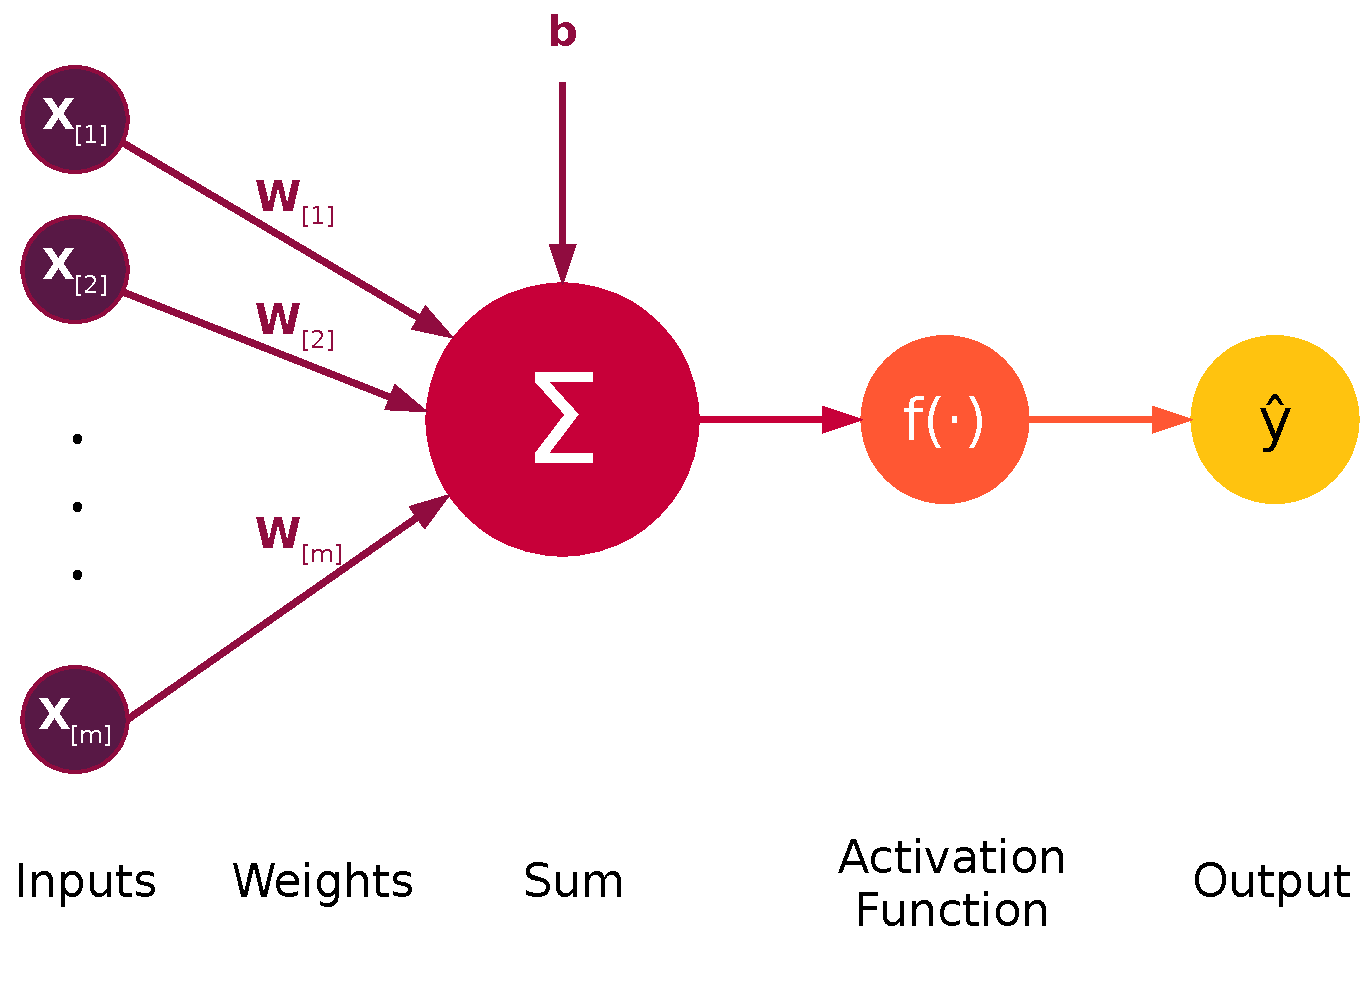
\includegraphics[width=\textwidth]{ch02-neuron-unit}
      \caption[Illustration of a neuron.]
      {Illustration of a neuron: each input value $\mathbf{x}_{[i]}$ is mapped
      to its corresponding weight $\mathbf{w}_{[i]}$.}
      \label{ch02:fig:neuron-unit}
    \end{figure}

    \pagebreak
    The activation function of a neuron usually depends on the task
    solved by the neural network model. Some functions are more suited for
    certain kinds of problems because they introduce non-linearity in the
    combination of the input values $\mathbf{x}_{[i]}$. Most commonly used
    activation function are plotted in~\autoref{ch02:fig:activation-function}.
    They are:
    \begin{itemize}
      \item Identity function: $f(x) = x$
      \item Sigmoid function: $f(x) = \frac{1}{1~+~e^{-x}}$
      \item Hyperbolic tangent function:
        $f(x) = \tanh(x) = \frac{e^x~-~e^{-x}}{e^x~+~e^{-x}}$
      \item ReLU function: $f(x) = \max(0, x)$
    \end{itemize}

    \begin{figure}[h!]
      \centering
      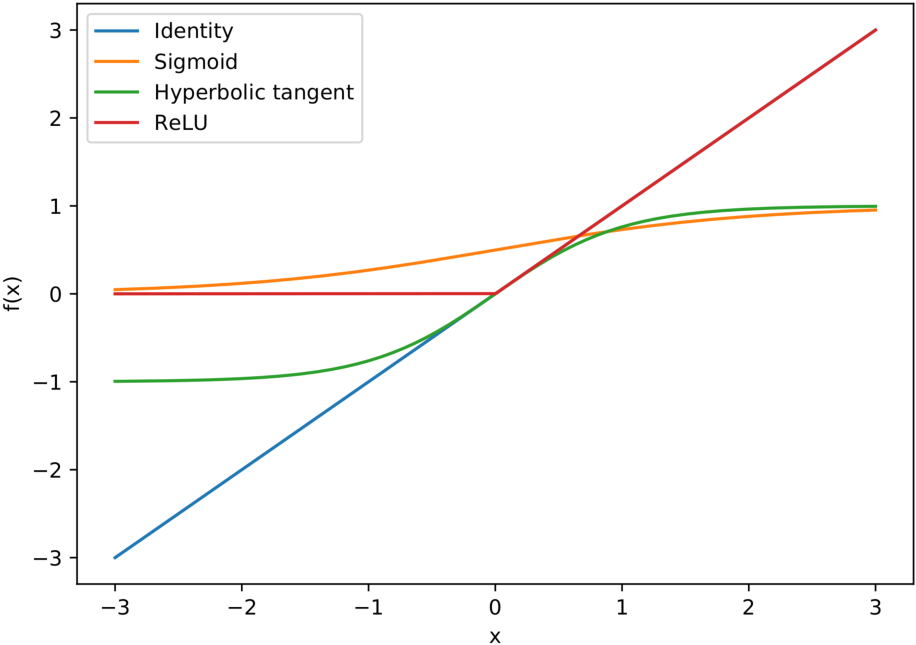
\includegraphics[width=\textwidth]{ch02-activation-function}
      \caption{Examples of activation functions found in a neuron.}
      \label{ch02:fig:activation-function}
    \end{figure}

    \medskip
    In a neural network, neurons are stacked up and linked together to form
    \textit{layers}.

    \theoremstyle{definition}
    \begin{definition}[A layer]
      A layer in a neural network is a group of neurons receiving the same input
      values. Layers are then cascaded so that the output values of a layer are
      the input values of the next layer. The first layer, which receives input
      values from data is the \textit{input layer}. The last layer which
      produces output value(s) of the network is the \textit{output layer}. Any
      layers between the input and the output layer are called \textit{hidden
      layers}.
    \end{definition}

    \noindent In~\autoref{ch02:fig:neural-network}, a multi-layer neural network
    is represented. It contains an input layer, an output layer and multiple
    hidden layers. Each layer has a specific number of neurons (the $i$-th layer
    has $d^i$ neurons). The neuron $\mathbf{n}_{i, j}$ is the $j$-th neuron of
    the $i$-th layer.

    \begin{figure}[t]
      \centering
      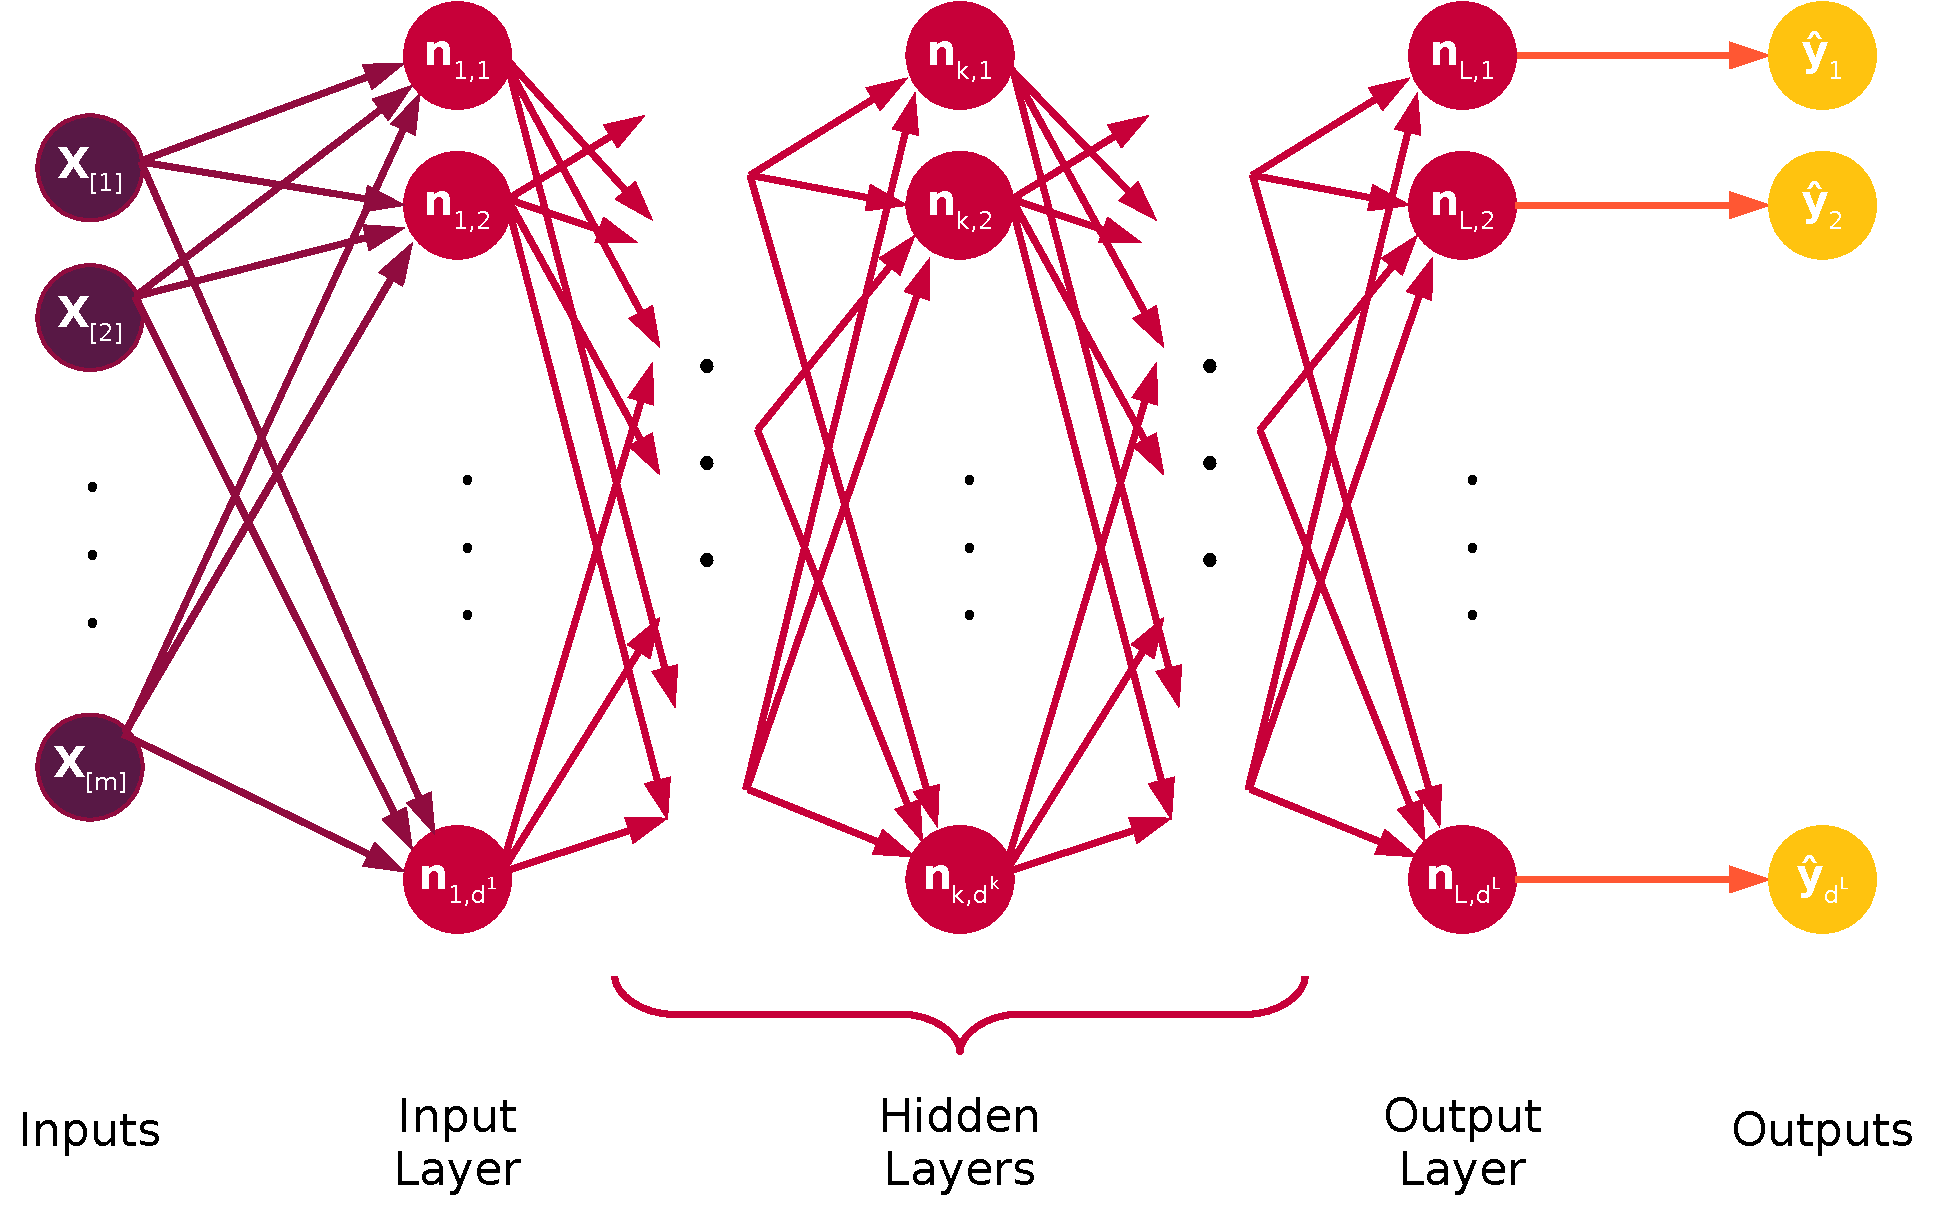
\includegraphics[width=\textwidth]{ch02-neural-network}
      \caption{Illustration of a multi-layer neural network.}
      \label{ch02:fig:neural-network}
    \end{figure}

    \pagebreak
    Neural networks are trained with supervised learning. They compute output
    values of given input labeled data and use a loss function (like the
    cross-entropy loss if the task is a multi-class classification problem) and
    the global loss on all the annotated examples to know if the predictions are
    correct or not. In a neural network, only the weights and biases are
    variable parameters (the activation function is chosen at the initialization
    of the neural network and is fixed during training). The optimal variable
    parameters $\Theta^*$ (weights and biases of neurons) that best solve the
    task are learned by the neural network by solving the following optimization
    problem:

    \begin{equation}
      \Theta^* = \argmin_{\Theta}~~\text{Global Loss  } (\Theta)
    \end{equation}
    The most common technique used to solve this optimization problem in neural
    networks is the gradient descent. Each parameter of the network has an
    influence on the value of the global loss because each variable parameter is
    used in the computation of the output value of its respective neuron and by
    forward propagation, used in the computation of the output values of the
    neural network. Each variable parameter is updated with the value of the
    derivative of the global loss with respect to this parameter. \medskip

    Neural networks are often used in NLP~\citep{zhang2015character,
    Xu2015convolutional, conneau2016very}. For example, in a classification
    task, input vectors can be the one-hot vectors of the words of a text and
    output values the probabilities of the text to belong to each possible
    class. The neural network \textit{learns} how to combine and weight each
    input word vector in order to predict the correct class.
    In~\autoref{chap:methods-we}, we will see how the architecture of neural
    networks can be modfied for the specific task of learning word embeddings.

  \subsection{Autoencoder}
    \label{ch02:subsec:autoencoder}
    Autoencoders are special kinds of neural networks. Similarly, they are also
    composed of an input layer and an output layer, but hidden layers have
    various sizes. \autoref{ch02:fig:autoencoder} represents the architecture of
    an autoencoder.

    \begin{figure}[t]
      \centering
      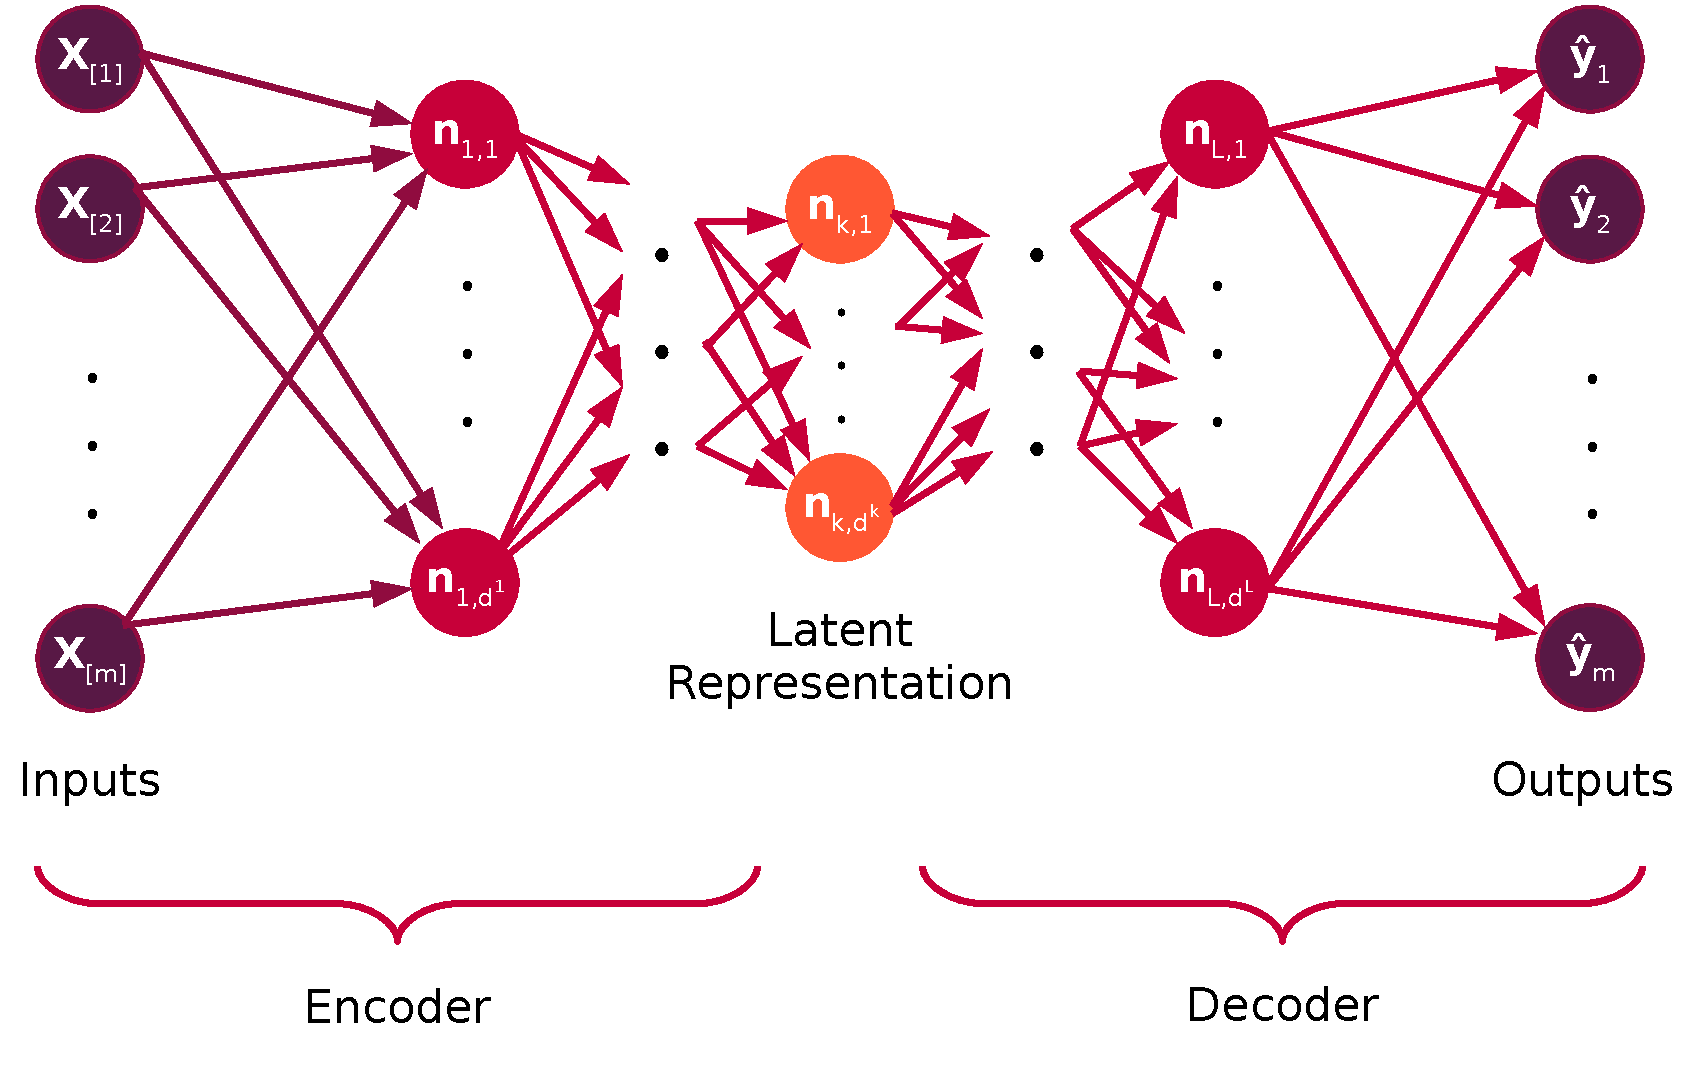
\includegraphics[width=\textwidth]{ch02-autoencoder}
      \caption[Illustration of an autoencoder.] {Illustration of an autoencoder.
      The decoder learns the latent representation which is used by the decoder
      to compute output values similar to input values.}
      \label{ch02:fig:autoencoder}
    \end{figure}

    First half of the layers of the autoencoder have a decreasing layer size,
    until the middle layer of the autoencoder. Second half of the layers have an
    increasing layer size, until the output layer. Output values $\hat{y}_k$ of
    an autoencoder are not predictions but values that aims to be as close as
    possible as the input vector values $\mathbf{x}_{[k]}$. Therefore, input and
    output layers must have identical size. Autoencoders are unsupervised models
    but trained like supervised models. However, they do not need any labels:
    they use a loss which compares output values to input vector values. A
    common loss used to train autoencoders is the quadratic loss, which is
    defined for each input vector as:

    \begin{equation}
      \text{Loss}(\mathbf{x}, \mathbf{\hat{y}})
        = \left\lVert \mathbf{x} - \mathbf{\hat{y}} \right\rVert^2
        = \sum_{i = 1}^m (\mathbf{x}_{[i]} - \hat{y}_i)^2
    \end{equation}
    Autoencoders are generally trained with the gradient descent technique to
    minimize the global loss on all the examples. The value of the derivative of
    the global loss with respect to each parameter of the model is used to
    update the value of parameters. \medskip

    Autoencoders are commonly used for dimensionality reduction (we will see
    in~\autoref{chap:methods-reduction} different methods to reduce the size of
    word embeddings, autoencoders are one of them). They are trained to learn a
    smaller representation of input data, but which contains enough information
    to \textit{reconstruct} the input data. Autoencoders are composed of two
    parts:

    \begin{enumerate}
      \item an encoder: composed of all the layers from the input layer to the
        middle hidden layer (the orange neurons
        in~\autoref{ch02:fig:autoencoder}). In the encoder part, the size of
        layers is only decreasing. The encoder can be seen as a function $\phi$
        that transforms an input vector $\mathbf{x} \in \mathbb{R}^m$ into a
        smaller vector $\ell \in \mathbb{R}^k$ which is called the
        \textit{latent representation}:

        \begin{equation}
          \phi: \mathbb{R}^m \to \mathbb{R}^k, m > k;~~\ell = \phi(\mathbf{x})
        \end{equation}

      \item a decoder: composed of all the layers from the middle hidden layer
        (the orange neurons in~\autoref{ch02:fig:autoencoder}) until the output
        layer. In the decoder part, the size of layers is only increasing. The
        decoder can be seen as a function $\psi$ that transforms a hidden
        representation $\ell \in \mathbb{R}^k$ into a vector $\mathbf{\hat{y}}
        \in \mathbb{R}^m$:

        \begin{equation}
          \psi: \mathbb{R}^k \to \mathbb{R}^m, k < m;~~\mathbf{\hat{y}} =
          \psi(\ell)
        \end{equation}
    \end{enumerate}

    The objective of an autoencoder is to compute output vectors
    $\mathbf{\hat{y}}$ as close as possible as input vectors $\mathbf{x}$,
    \textit{i.e.} to learn $\phi$ and $\psi$ that mimimize $\left\lVert
    \mathbf{x} - \mathbf{\hat{y}} \right\rVert$ for all the data vectors
    $\mathbf{x} \in \mathcal{S}$. In other terms, to solve the following
    optimization problem:

    \begin{equation}
      \argmin_{\phi, \psi} \sum_{\mathbf{x} \in \mathcal{S}}
                    \left\lVert \mathbf{x} - \psi(\phi(\mathbf{x})) \right\rVert
    \end{equation}
    The hidden representation $\ell$, called the \textit{latent representation},
    has less dimensions than the input vector $\mathbf{x}$, but the decoder part
    only uses this latent representation to produce $\mathbf{\hat{y}}$.
    Therefore, the autoencoder has to learn a latent representation which
    contains enough information to produce a vector $\mathbf{\hat{y}}$ close to
    the input vector $\mathbf{x}$. In an autoencoder, both parts work jointly:
    the encoder learns which values of the input vector are the most important
    to keep and transform into the latent representation while the decoder tells
    the encoder if its choices are good enough to reconstruct the input vector.

\section{Conclusion}
  Machine learning models are great tools to solve problems automatically.
  Their main advantage is that they can find by themselves what is the
  information encoded in data representations required to solve the problem,
  without any human interactions to indicate what are the steps to follow. When
  they are used in the NLP domain, they can solve problems like translating
  documents, classifying texts into the correct category or grouping together
  people with similar style of writing. \medskip

  In this chapter, we have described what is machine learning and what are the
  differences between the two main types of machine learning algorithms:
  supervised learning uses labeled data to learn how to map inputs to outputs
  while unsupervised learning learns about the distribution of information in
  data. We have also presented the most common models used to learn word
  embeddings, which are neural networks and autoencoders, and we have explained
  how they learn from data to solve a given problem. \medskip

  However, in~\autoref{chap:preliminaries}, we have explained that finding
  numerical representations for words is an important preliminary step when
  solving NLP tasks, because good representations that encode a large amount of
  linguistic information is useful for the downstream machine learning model: if
  this downstream model has access to more relevant information, it can better
  understand data and make better predictions. Which raises the following
  question: how can machine learning models be used to learn good word
  representations?  This is the main topic of the next chapter.
  In~\autoref{chap:methods-we}, we present a detailed review of the existing
  methods to learn word embeddings and the characteristics of each method.
